\documentclass[../Elmag-labhefte-2020.tex]{subfiles}

\begin{document}


\chapter{LORENTZKRAFTEN \label{ch.lorentz}}

\subsection*{Mål}

Du skal i denne laboratorieoppgaven
%
\begin{itemize}
    \item dokumentere eksperiment i labjournalen
    \item foreta feilanalyse av eksperimentet.
    \item bruke numeriske metoder for å modellere eksperimentet
    \item studere krefter på elektroner i homogene og konstante elektriske og magnetiske felt,
    \item bestemme forholdet $e/m$ mellom elektronets ladning $e$ og masse $m$ (Thomsoneksperimentet),
\end{itemize}
%

%**********************************************
\section{Teoretisk bakgrunn}
%**********************************************

Teorien presenteres i samband med presentasjonen av beregningsoppgavene nedenfor. Det vises også til lærebok og forelesningene i elektromagnetisme.

%%%%%%%%%%%%%%%%%%%%%%%%%%%%%%%%%%%%%%%%%%%%%%%%%%%
\section{Beregningsoppgaver \label{ch.lorentz.beregn}}
%%%%%%%%%%%%%%%%%%%%%%%%%%%%%

\subsection{Lorentzkraften}
%**********************************************

Kraften fra elektriske og magnetiske felt på ladde partikler kalles gjerne Lorentzkraften. Kraften på en ladd partikkel med ladning $q$ som beveger seg med hastighet $\vec{v}$ i et elektrostatisk felt $\va*{E}$ og et magnetostatisk felt $\va*{B}$ er gitt ved 
\begin{equation}
    \va*{F} = q \va*{E} + q \va*{v} \cross \va*{B} .
    \label{eq:lorentz.lorentz} %(3)
\end{equation}
%
For å lage en hurtig elektronstråle brukes alltid elektriske felt for å akselerere elektronene. Uttrykket for Lorentzkraften viser imidlertid at både elektriske og magnetiske felt gir kraftvirkning på ladde partikler. 

{\itsf 1. Forklar ut i fra uttrykket for Lorentzkraften hvorfor magnetiske felt (i motsetning til elektriske felt) ikke kan gi en ladd partikkel økt kinetisk energi.}

\subsection{Ladninger i \textsl{E}-felt}
%**********************************************

Et homogent elektrisk felt settes lettest opp mellom to parallelle plateleektroder. Denne geometrien gir et elektrisk felt $E = U_\mathrm{a}/\ell$ hvor $U_\mathrm{a}$ er spenningen mellom platene og $\ell$ avstanden mellom dem. En ladd partikkel med ladning $q$ og masse $m$ blir under passasje mellom platene akselerert med en akselerasjon 
\begin{equation}
    a = \frac{q E}{m} = \frac{q U_\mathrm{a}}{m\ell}.
    \label{eq:lorentz.aksel}
\end{equation}
%
Dette anvendes i kilder for ladde partikkelstråler. 

Figur \ref{lorentz.fig1} viser hvordan en elektronstrålekilde kan lages. Et wolfram-filament varmes opp ved at elektrisk strøm passerer gjennom det. Når det er rødglødende sender det ut elektroner fra overflata. Filamentet plasseres like bak en plateelektrode med hull i. Spenning legges mellom filamentet og plateelektroden. Elektronene blir akselerert mot plateelektroden og de elektronene som passerer hullet går ut i en stråle på andre siden av plata. En annen måte å lage elektroner i elektronkilder er å bruke en oksidkatode som blir varmet opp indirekte av et filament. Denne konstruksjonen gir bedre feltforhold under akselerasjonen, og det er denne utgaven som er vist i figur \ref{lorentz.fig1}.
%

\begin{figure}[!h]
    %\setlength{\unitlength}{1mm}
    \vspace{-2cm}
    %\begin{picture}(60,60)(0,0)
    %\put(58.5,76){\large \sf 1}
    %\put(56,73){$\overbrace{}$}
    %\put(47,55.5){\vector(1,0){29}}
    %\put(44,54){\large \sf 2}
    %\put(55,53){\vector(1,0){28}}
    %\put(52,51){\large \sf 3}
    %\put(90,73){\vector(0,-1){20}}
    %\put(88,75){\large \sf 4}
    \centering
    \includegraphics[width=9cm,height=8cm,keepaspectratio]{fig/LorentzFig1_resized.pdf}
    %\end{picture}
    %\vspace{-2cm}
    \caption{%
        Prinsippskisse for elektronstrålekilde. 
        (1) Vekselspenning (5-\SI{10}{\volt}) til 
        (2) glødefilament varmer opp 
        (3) oksidbelegget. 
        Akselerasjonsspenning mellom filamentet og 
        (4) anoden akselerer elektronene.
    }
    \label{lorentz.fig1}
\end{figure}

Anta at et elektron blir akselerert fra stillstand til en spenning på \SI{30}{\volt} i et statisk elektrisk felt. 

{\itsf 2. Hva blir hastigheten til elektronet etter akselerasjonen? }

I partikkelakseleratorfysikk brukes energienheten "elektronvolt", forkortet \si{\eV}. En partikkel ladd med en elementærladning får energien 1 eV når den akselereres gjennom et spenningsfall på \SI{1}{\volt}.  

{\itsf 3A.  Hvor mange joule tilsvarer \SI{1}{\eV}? } 

{\itsf 3B.  Hva blir energien til et elektron som akselereres til en spenning på \SI{30}{\volt} uttrykt i enheten \si{\eV}?}
 
En elektronstråle fra en elektronkilde med null potensial blir akselerert til et potensial $U_\mathrm{a}$ vil kunne avbøyes i et transversalt elektrisk felt $E = U_\mathrm{d} /d$ over en avstand $L$ som vist i figur \ref{lorentz.fig2}. Avbøyningsvinkelen $\alpha$ er gitt av
\begin{equation}
    \tan \alpha = \half \frac{U_\mathrm{d}}{U_\mathrm{a}}  \frac{L}{d} .
    \label{eq:lorentz.5}
\end{equation}

\begin{figure}[!h]
    \setlength{\unitlength}{1mm}
    \begin{picture}(100,65)(0,0)
        \multiput(30,40)(2.5,0){12}{\line(1, 0){2}}%horizontal dashed
        \multiput(60,40)(4.3,0.86){14}{\line(5, 1){3.6}}%inclined dashed
        \put(60, 40){\line(1, 0){60}
        \linethickness{0.3mm}
        \put(0, -20){\line(0, 1){40}}}%screen
        %\color{red}
        \linethickness{0.1mm}
        %%%%%%%%%%%%%%%
        \put(120, 41){\Large$\downarrow$}
        \put(120, 48){\Large$\uparrow$}
        \put(121.5, 44){\line(0, 1){4}}
        \put(122, 45){\large$\Delta y$}
        \put(112, 61){\sf skjerm}
        %%%%%%%%%%%%%%
        
        \qbezier(86.5,45)(88,43)(87,40)
        \put(88, 42){$\alpha$}
        %%%%%%%%%%%%%%
        \color{black}
        \put(60, 43){\line(0, 1){10}}%upper plate lead
        \put(60, 37){\line(0, -1){10}}%lower plate lead
        \linethickness{0.3mm}
        \put(53, 37){\line(1, 0){14}}%lower plate
        \put(53, 43){\line(1, 0){14}}%upper plate
        %\color{red}
        %\put(40,30){\tiny$\bullet$}
        %\put(40,50){\tiny$\bullet$}
        %\put(46,36){\tiny$\bullet$}
        %\put(46,44){\tiny$\bullet$}
        \qbezier(40,30)(43,33)(46,36)
        \qbezier(40,50)(43,47)(46,44)
        
        \put(30,35){\line(0, 1){10}}
        \put(30,35){\line(-1, 0){4}}
        \put(30,45){\line(-1, 0){4}}
        \linethickness{0.1mm}
        %%%%%%%%%
        \put(25.6,40.5){$\exists$}
        \put(25.6,36.5){$\exists$}
        \put(27.6,36.5){\line(0, 1){4}}
        \put(22,52){\sf elektron-}
        \put(22,47){\sf kanon}
        %%%%%%%%%
        \put(26,36.5){\line(0, -1){13.5}}
        \put(26,23){\line(1, 0){4}}
        \put(43,33){\line(0, -1){10}}
        \put(43,23){\line(-1, 0){4}}
        %%%%%%%%%%%
        \put(30,22){$\underbrace{}_{\sf 2.0\; kV}$}
        \put(28,24){$-$}
        \put(37.5,24){$+$}
        
        \put(56,34){$-$}
        \put(56,46){$+$}
        \put(62,45.5){\sf 20\;V}
        
        %%%%%%%%%%%
        \put(52,46){\line(0, 1){8}}
        \put(51, 44){$\downarrow$}%upper plate downarrow
        \put(51, 34){$\uparrow$}%upper plate uparrow
        %\put(51, 48){$d$}
        \put(45,55){$d={\sf 2.0\; cm}$}
        \multiput(53, 36.4)(0,-2.5){6}{\line(0, -1){1}}%lower plate
        \multiput(67, 36.4)(0,-2.5){6}{\line(0, -1){1}}%lower plate
        \put(51.5,22){$\underbrace{\qquad\qquad}_{L={\sf 5.0\; cm}}$}
        %%%%%%%%%
        
        \put(90, 34.6){\vector(-1, 0){30}}%lower plate lead
        \put(90, 34.6){\vector(1, 0){30}}%lower plate lead
        \put(80,30){$L_\mathrm{s}={\sf 25\; cm}$}
        
    \end{picture}
    \vspace{-1cm}
    \caption{%
        Avbøyning av elektronstråle i et elektrisk felt. Tallverdier i figuren brukes i oppgaven.
    }
    \label{lorentz.fig2}
\end{figure}

Likning \eqref{eq:lorentz.5} beskriver de fysiske lover som danner grunnlaget for oscilloskopet, som er et instrument for måling av elektrisk spenning. Spenningen som skal måles legges mellom de transversale avbøyningsplatene og avbøyningen av elektronstrålen observert på en fosforescerende skjerm er et mål for spenningen. 

%Oscilloskopet omhandles seinere i seminar i kapittel \ref{ch.oscilloskop}. Her utledes også likningen (\ref{eq:lorentz.5}), se likning (\ref{osc.6}) side \pageref{osc.6}

Anta elektronene blir akselerert av et \SI{2}{\kilo\volt} akselerasjonspotensial og de øvrige parametre er som vist i figur \ref{lorentz.fig2}. 

{\itsf 4.  Hvor stor avbøyning $\Delta y$ får strålen på skjermen hvis avbøyningsspenningen er \SI{20}{\volt}?}

\subsection{Ladninger i \textsl{B}-felt}
%**********************************************

Når et elektron beveger seg i et rom fritt for elektrisk felt men med et magnetisk felt $B$ virker Lorentzkraften til enhver tid normalt på baneretningen (så sant ikke banen er parallell med magnetfeltet). La oss anta elektronet skytes inn i $B$-feltet med hastighet vinkelrett på feltet, Lorentzkraften blir da $F_\mathrm{B} = evB$ og utgjør sentripetalkraften. Elektronbanen blir en sirkel med radius $r$ med sentripetalakselerasjon $a_\mathrm{s} = v^2/r = F_\mathrm{B}/m$. Farten $v$ kan bestemmes fra den kinetiske energien til elektronet gitt av $\half mv^2 = e U_\mathrm{a}$. Ved å sette sammen disse likningene får vi følgende uttrykk for radien
\begin{equation}
    r = \frac{1}{B} \sqrt{\frac{2 U_\mathrm{a}}{e/m}} .
    \label{eq:lorentz.6}
\end{equation}

{\itsf 5.  Sett opp i et kurvediagram kurveskarer over $r$ sfa. $B$ i området $0 < B < \SI{15}{\gauss}$ for $U_\mathrm{a} = 20$, \num{40} og \SI{60}{\volt}}. Bruk for eksempel Python eller Matlab.


\subsection{Bestemmelse av \textsl{e/m} (Thomsoneksperimentet)}
%**********************************************
 
I 1897 oppdaget Thomson
%\footnote{Sir Joseph John Thomson (1856-1940), britisk fysiker. Nobelpris i fysikk 1906 for undersøkelser av elektrisk ladning i gasser.} 
ekstremt lette, negativt ladde partikler -- som senere viste seg å være elektroner. Samme år brukte han avbøyning i statiske elektriske og magnetiske felt til å finne forholdet mellom deres ladning og masse. Uttrykket \eqref{eq:lorentz.6} kan omskrives til 
\begin{equation}
    \frac{e}{m} = \frac{2 U_\mathrm{a}} {B^2 r^2}.
    \label{eq:lorentz.7}
\end{equation}
%
Forholdet $e/m$ kan altså bestemmes ved å måle radius $r$ i elektronbanen i et magnetfelt $B$ vinkelrett på banen for elektroner akselerert over en spenning $U_\mathrm{a}$. 

Du skal gjenta Thomsons eksperiment i laboratoriet. Størrelsen på apparaturen begrenser diameteren på største elektronbane til ca. \SI{8}{\cm}. 

{\itsf 6.  Bruk kurveskaren som du satt opp i oppgaven ovenfor til å anslå gunstig magnetfelt $B$ for tre ulike akselerasjonsspenninger $U_\mathrm{a} = 20$, \num{40} og \SI{60}{\volt}.}
 
Ved omskrivning av \eqref{eq:lorentz.7} får du 
\begin{equation}
    m = \frac{q B^2 r^2}{2 U_\mathrm{a}},
    \label{eq:lorentz.8}
\end{equation}
%
som viser at massen $m$ til en ladd partikkel med kjent ladning $q$ som har vært akselerert til et kjent potensial $U_\mathrm{a}$ kan bestemmes ved å måle magnetisk flukstetthet $B$ og baneradius $r$ for partikkelen i et magnetisk felt. Dette er ideen bak det magnetostatiske massespektrometeret som er et av de viktigste instrumentene for bestemmelse av atomære og molekylære partikkelmasser. Thomson la med sitt arbeid grunnlaget for denne teknikken.

\subsection{Spenningsdeler \label{lorentz.spenningsdeler}}
%**********************************************
 
Den såkalte spenningsdeleren er blant de mest alminnelige elektriske oppkoplinger. Du skal anvende den i eksperimentet. I sin enkleste form ser spenningsdeleren ut som i figur \ref{lorentz.fig3}A.

\begin{figure}[!ht]
    \setlength{\unitlength}{0.75mm}
    \begin{picture}(180,65)(-10,0)
        \newsavebox{\ResistorSV}%Resistor Short Vertical
        \savebox{\ResistorSV}(0,0)[l]{%
            \multiput(14, 48)(0,-2.2){4}{\footnotesize$>$}%
            \qbezier(14.5,50.5)(15,51)(15.5,51.5)
            \qbezier(14.5,41.5)(15,41)(15.5,40.5)
            \put(15.5,51.5){\line(0, 1){3.5}}
            \put(15.5,40.5){\line(0, -1){3.5}}
        }
        \put(0,-4.5){\usebox{\ResistorSV}}
        
        \put(5,4.5){\tiny$\bullet$}
        \put(5,5){\line(1, 0){25}}%bottom line
        \put(30,4.5){\tiny$\bullet$}
        
        %%%%%%%%%%%
        \put(5,54.5){\tiny$\bullet$}
        \put(5.5,55){\line(1, 0){10}}
        %%%%%%%%%%%%%
        
        \put(15,29.5){\tiny$\bullet$}
        \put(15,30){\line(1, 0){15}}
        \put(30,29.5){\tiny$\bullet$}
        %%%%%%%%%%%%%%%
        %\linethickness{0.3mm}
        \multiput(14, 48)(0,-2.2){4}{\footnotesize$>$}%
        \qbezier(14.5,50.5)(15,51)(15.5,51.5)
        \qbezier(14.5,41.5)(15,41)(15.5,40.5)
        \put(15.5,51.5){\line(0, 1){3.5}}
        \put(15.5,40.5){\line(0, -1){20}}
        %%%%%%%%%%%%%%%
        
        \put(5,35){\vector(0, 1){20}}
        \put(0,30){$V_\mathrm{inn}$}
        \put(5,25){\vector(0, -1){20}}
        
        \put(30,20){\vector(0, 1){10}}
        \put(30,15){$V_\mathrm{ut}$}
        \put(30,15){\vector(0, -1){10}}
        
        \put(18,45){$R_{1}$}
        \put(18,12){$R_{2}$}
        %%%%%%%%%%%
        \put(60,4.5){\tiny$\bullet$}
        \put(60,54.5){\tiny$\bullet$}
        \put(60,5){\line(1, 0){35}}
        \put(60,55){\line(1, 0){15}}
        
        \newsavebox{\ResistorLV}%Resistor Long Vertical
        \savebox{\ResistorLV}(0,0)[l]{%
            \multiput(14, 48)(0,-2.2){12}{\footnotesize$>$}%
            \qbezier(14.5,50.5)(15,51)(15.5,51.5)
            \qbezier(14.5,23.5)(15,23)(15.5,22.5)
            \put(15.5,51.5){\line(0, 1){3.5}}
            \put(15.5,22.5){\line(0, -1){10}}
        }
        \put(59.5,20){\usebox{\ResistorLV}}
        \put(75,55){\line(0, -1){10}}
        
        \put(95,4.5){\tiny$\bullet$}
        \put(95,29){\tiny$\bullet$}
        \put(79,29.5){\line(1,0){16}}
        \put(75,28){\large$\lhd$}  %\put(75,28){\large$\longleftarrow\!\!\!-\!\!\!-\!\!\!-$}
        \multiput(80, 23)(0,2.5){6}{\line(0, 1){1}}
        \put(78.6,21.6){\tiny$\bigtriangledown$}
        \put(78.6,36.7){\tiny$\bigtriangleup$}
        \put(67,35){$R_{1}$}
        \put(67,22){$R_{2}$}
        
        \put(60,35){\vector(0, 1){20}}
        \put(55,30){$V_\mathrm{inn}$}
        \put(60,25){\vector(0, -1){20}}
        
        \put(95,20){\vector(0, 1){10}}
        \put(95,15){$V_\mathrm{ut}$}
        \put(95,15){\vector(0, -1){10}}
        %
        %%%%%%%%%%%%%%%%%
        %\put(115,4.5){\tiny$\bullet$}
        %\put(115,54.5){\tiny$\bullet$}
        %\put(115,5){\line(1, 0){30}}
        %\put(115,55){\line(1, 0){10}}
        
        \newsavebox{\VoltageDivider}
        \savebox{\VoltageDivider}(0,0)[l]{
            \put(60,4.5){\tiny$\bullet$}
            \put(60,54.5){\tiny$\bullet$}
            \put(60,5){\line(1, 0){35}}
            \put(60,55){\line(1, 0){15}
        }
        
        \put(59.5,20){\usebox{\ResistorLV}}
        \put(75,55){\line(0, -1){10}}
        
        \put(95,4.5){\tiny$\bullet$}
        \put(95,29){\tiny$\bullet$}
        \put(79,29.5){\line(1,0){16}}
        \put(75,28){\large$\lhd$} %\put(75,28){\large$\longleftarrow\!\!\!-\!\!\!-\!\!\!-$}
        %\multiput(80, 23)(0,2.5){6}{\line(0, 1){1}}
        %\put(78.6,21.6){\tiny$\bigtriangledown$}
        %\put(78.6,36.7){\tiny$\bigtriangleup$}
        \put(67,35){$R_{1}$}
        \put(67,22){$R_{2}$}
        
        \put(60,35){\vector(0, 1){20}}
        \put(55,30){$V_\mathrm{inn}$}
        \put(60,25){\vector(0, -1){20}}
        
        \put(95,20){\vector(0, 1){10}}
        \put(95,15){$V_\mathrm{ut}$}
        \put(95,15){\vector(0, -1){10}}
        }
        
        \put(70,28){\usebox{\VoltageDivider}}
        \put(159.6,0){\usebox{\ResistorSV}}
        \put(165,5){\line(1, 0){10}}
        \put(165,30){\line(1, 0){10}}
        \put(175,5){\line(0, 1){5}}
        \put(175,30){\line(0, -1){5}}
        \put(178,15){$R_\mathrm{L}$}
        \put(10,60){\large \sf A}
        \put(60,60){\large \sf B}
        \put(130,60){\large \sf C}
    \end{picture}
    %\vspace{-1cm}
    \caption{%
        Spenningsdeler. 
        (A) Med faste motstander. 
        (B) Med variabel motstand med midttapping (skyvemotstand/potensiometer). 
        (C) Med potensiometer og last $R_\mathrm{L}$.}
    \label{lorentz.fig3}
\end{figure}
%

%
Gjennom koplingen kan spenningen $V_\mathrm{inn}$ reduseres til $V_\mathrm{ut}$. For å finne størrelsen på $V_\mathrm{ut}$ sfa. $V_\mathrm{inn}$ kan du se på strømmen $I$ gjennom motstandene $R_1$ og $R_2$ som ifølge Ohms lov er lik
\begin{equation}
    I = \frac{V_\mathrm{inn}}{R_1 + R_2} .
\end{equation}
Bruk Ohms lov igjen på $R_2$:
\begin{equation}
    V_\mathrm{ut} 
        = I  R_2 
        = \frac{R_2}{R_1 + R_2} V_\mathrm{inn}.
\end{equation}
Spenningsdeleren kan gjøres variabel ved å erstatte $R_1$ og $R_2$ med en motstand med variabel midttapping (skyvemotstand) som vist på figur \ref{lorentz.fig3}B. Sammen med en fast spenningskilde gir dette en mulighet til å lage en billig variabel spenningskilde. 

Spenningsdeleren har imidlertid en ulempe. 

{\itsf 7. Kan du finne hvilken ulempe? }
\\
TIPS: Hva  skjer med $V_\mathrm{ut}$ når du begynner å trekke strøm fra utgangen (midttappingen)? Se figur \ref{lorentz.fig3}C. Resultantmotstanden over parallellkoplingen av $R_2$ og $R_\mathrm{L}$ betegnes $R_2||R_\mathrm{L}$ og er lik $ (R_2R_\mathrm{L})/(R_2 + R_\mathrm{L})$.


%\newpage

%%%%%%%%%%%%%%%%%%%%%%%%%%%%%%%%%%%%%%%%%%%%%%%%%%%%%%%%%%%%%%%%%%%%%%%%%%%%%%
\section{Eksperimentelt \label{ch.lorentz.eksp} }
%%%%%%%%%%%%%%%%%%%%%%%%%%%%%%%%%%%%%%%%%%%%%%%%%%%%%%%%%%%%%%%%%%%%%%%%%%%%%%

%%%%%%%%%%%%%%%%%%%%%%%%%%%%%%%%%%%%%%%%%%%%%%%%%%%%%%%%%%%%%%%%%%%%%%%%%%%%%%
\subsection{Apparatur}
%%%%%%%%%%%%%%%%%%%%%%%%%%%%%%%%%%%%%%%%%%%%%%%%%%%%%%%%%%%%%%%%%%%%%%%%%%%%%%

\vspace{-4mm} 
\begin{itemize}
    \item \textbf{Elektronstrålerør.} Leybold Hereaus 555 571.
    \item \textbf{Kraftforsyning for elektronakselerasjonen og fokuseringselektrode.} Leybold Didactics 521 651	Tube power supply 0...500 V.
    
    \item \textbf{Kraftforsyning for Helmholtzspoler.} Mascot, type 719.  Brukes som strømkilde. 
    Område: 0-\SI{15}{\volt}, \SI{30}{\milli\ampere}-\SI{2}{\ampere}.
    \item \textbf{Multimeter for spolestrøm.} Escort EDM168A, 3 sifre, eller tilsvarende.
    % Presisjon: 3 sifre.
    \item \textbf{Multimeter for akselerasjonsspenning.} Escort EDM168A, 3 sifre, eller tilsvarende.
    % Presisjon: 3 sifre.
   
    \item \textbf{Koplingsboks B med spenningsdeler.}
    \item En mengde \textbf{ledninger} av ulik lengde.
\end{itemize}

\begin{figure}[ht]
    \begin{minipage}[b]{0.45\linewidth}
        \centering
        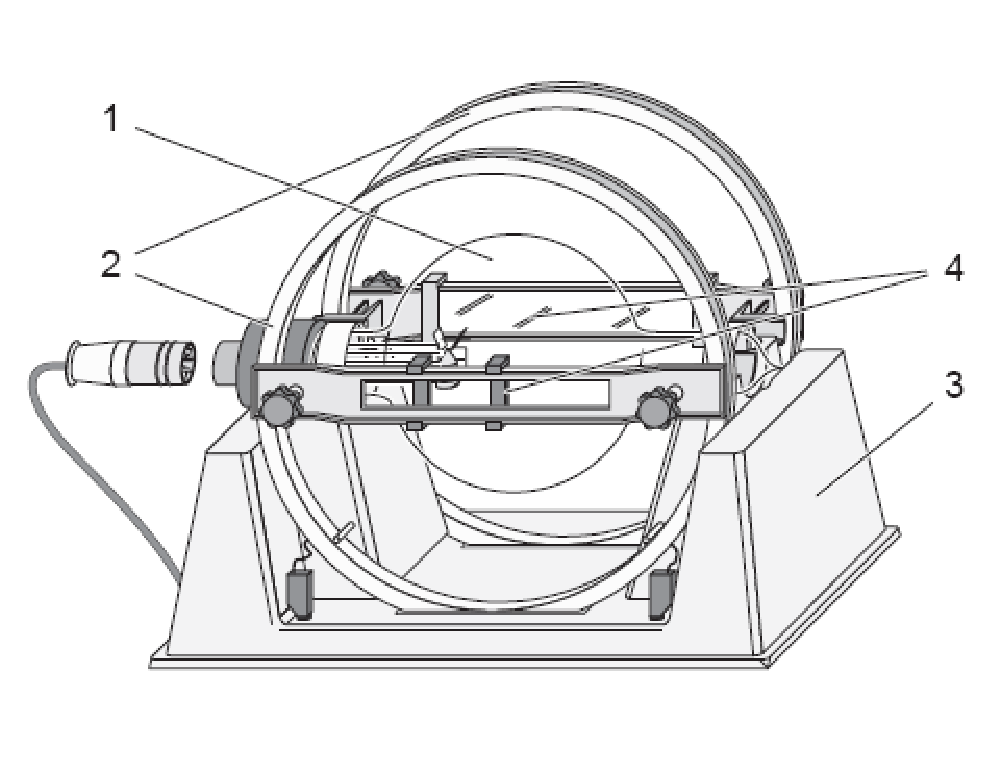
\includegraphics[scale=0.525]{fig/FineBeamApparat.eps}
        \caption{%
            Leybold apparat med elektronkanonen innen glasskolbe (1), 
            Helmholtzspoler (2), 
            holder (3), 
            og radiusmåler (4).
        }
        \label{lorentz.fig4}
        \vspace{0.5cm}
    \end{minipage}
    \hspace{1cm}
    \begin{minipage}[b]{0.5\linewidth}
        \centering
        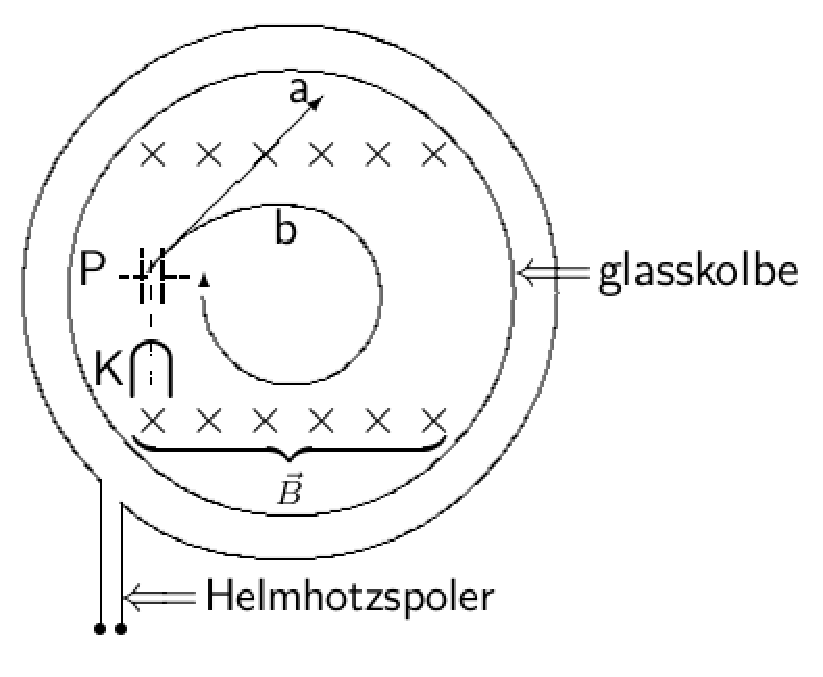
\includegraphics[scale=0.525]{fig/Schematic.eps}
        \caption{%
            Prinsippskisse. 
            Elektronkanonen (K), 
            avbøyning av elektronstrålen mellom avbøyningsplater (P). 
            Magnetfelt er markert med kryss $\times$ \textsl{inn i} papirplanet og elektronstrålen er vist uten (a) og med $B$-felt (b). }
        \label{lorentz.fig5}
    \end{minipage}
\end{figure}
Apparaturen er vist skjematisk i figurene \ref{lorentz.fig4} og  \ref{lorentz.fig5}. Elektronkanonen (\textsf{K}) sender ut elektroner som kan avbøyes i et statisk elektrisk felt mellom de parallelle avbøyningsplatene (\textsf{P}) og/eller i et statisk magnetfelt fra Helmholtzspolene. Glasskolben rundt elektronkanonen er fylt med tynn hydrogengass til et trykk på omtrent \num{e-5} atmosfærer \SI{1}{\pascal}. Støt mellom elektronene og gassen vil eksitere elektronene i gassmolekylene som så deeksiterer og sender ut lys (samme fenomen som ved nordlys). Sporet etter elektronene blir da synlig som en blågrønn stripe. 

{\itsf Studer elektronkanonen gjennom glasskolben. Studer også den demonterte kanonen fra et gammelt rør som er utlagt i laboratoriet.}
\newpage
\subsection{Oppkopling av spenninger til elektronkanonen}
%%%%%%%%%%%%%%%%%%%%%%%%%%%%%%%%%%%%%%%%%

Figurene \ref{lorentz.fig6} og \ref{lorentz.fig7} viser skjematisk de elektriske oppkoplinger for elektronkanonen. Notera den gemensamma jordningpunkten (utgång 2 på Leybold Power supply)

\begin{figure}[!ht]
    \vspace{-9em}
    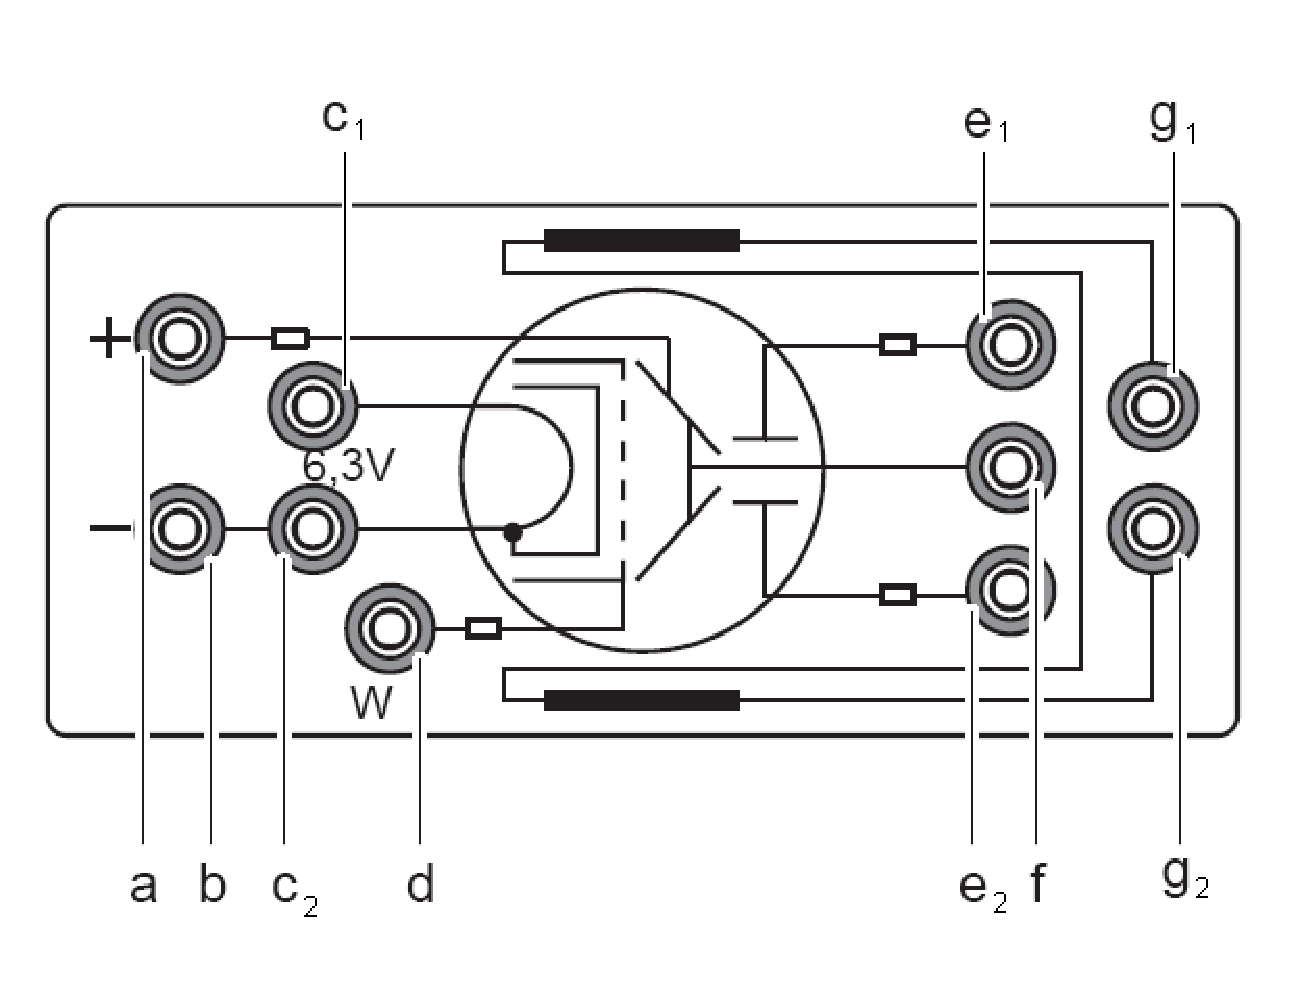
\includegraphics[width=0.55\textwidth]{LorentzCirc0}
    \begin{minipage}[b]{0.42\textwidth}
        \textsf{%
            a: anodespenning,\\
            b: jordingspunkt,\\
            c: glødespenning til katoden,\\
            d: Wehneltsylinder,\\
            e: avbøyningsspenning (øvre og nedre),\\
            f: punkt for måling anodespenning,\\
            g: strømtilførsel Helmholtzspoler.
            \vspace{15mm}
        }
    \end{minipage}
    \caption{%
        Elektrisk tilkoplingskjema på apparaturens sidekant.
    }
    \label{lorentz.fig6}
\end{figure}

\begin{figure}[!ht]
    \centering
    \includegraphics[width=14cm,height=9.49cm,keepaspectratio]{fig/Lorentz03-New.pdf}
    \caption{%
        Koplingsskjema for elektronkanonen. Kraftforsyning Leybold, multimeter for måling av anodespenning.
    }
    \label{lorentz.fig7}
\end{figure}

Det finnes flere alternative måter å kople opp elektronkanonen, men det er viktigt att koble rett. Det er imidlertid ikke vanskelig å ødelegge et par sikringer om du kopler feil, så spør veileder dersom du er i tvil.

{\itsf Kople opp glødekretsen i henhold til figur \ref{lorentz.fig7}.}

Merknader og tips:
\vspace{-4mm} 
\begin{itemize}
    \item Du skall koble till uttak 4 på aggregatet. Vilken du bruker er utan betydelse men en jordas via kontakterna b och c$_1$ i figur \ref{lorentz.fig6}.
    \item Aggregatet skal være avslått under oppkopling. 
    \item Be labveilederen om å godkjenne oppkoplingen.
    \item Slå på aggregatet og juster glødspenningen til "6"(V) og observer at tråden gløder. Dette forutsetter at takbelysningen er slått av og bordbelysningen dempet. Observer at glødspenningen kan senkes til 5 V under eksperimentene.
    \item Slå aggregatet av igjen.
\end{itemize}

%\begin{figure}[!ht]
%    \begin{center}
%    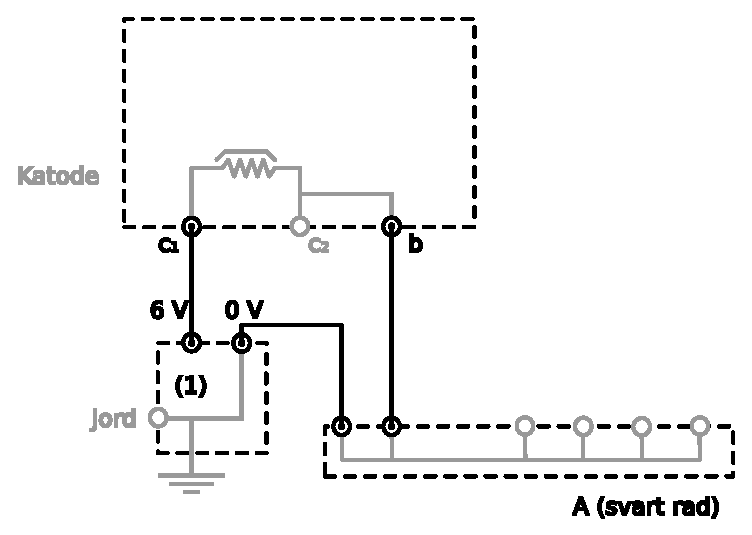
\includegraphics[width=0.6\textwidth]{glodekrets.eps}
%    \caption{%
%        Kretsdiagram for elektronkanonen, steg 1: oppkopling av glødekretsen. De delene av diagrammet som er innenfor de stiplede rektanglene illustrerer interne koplinger som du hverken kan eller trenger gjøre noe med. Bokstavene ved inngangene til elektronkanonen (det øverste stiplede rektangelet) viser til tilkoplingspunktene i figur \ref{lorentz.fig6}. Det stiplede rektangelet nede til høyre representerer den svarte raden med tilkoplingspunkter på koplingsboks A, og (1) representerer transformatoren.
%    }
%    \label{fig:glodekrets}
%    \end{center}
%\end{figure}

%\begin{figure}[!ht]
%    \begin{center}
%    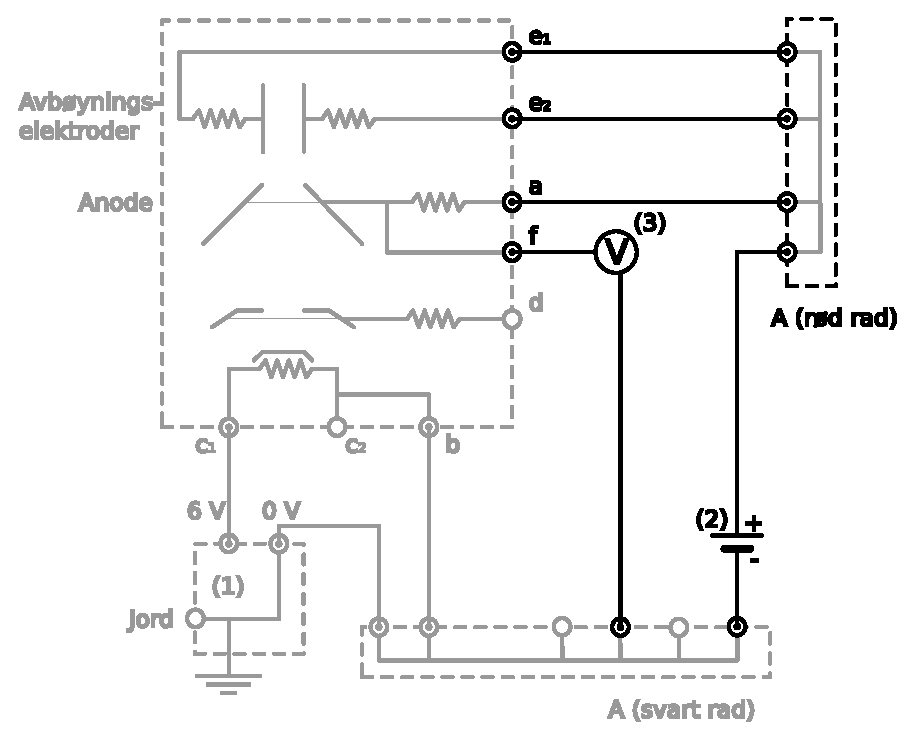
\includegraphics[width=0.6\textwidth]{anodespenning.eps}
%    \caption{%
%        Kretsdiagram for elektronkanonen, steg 2: tilkopling av anoden. De delene av diagrammet som har lysere farge er allerede oppkoplet i forrige steg; se forøvrig figur \ref{fig:glodekrets} for forklaring. Det stiplede rektangelet oppe til høyre representerer den røde raden med tilkoplingspunkter på koplingsboks A, (2) representerer Delta Elektronika kraftforsyning, og (3) representerer et multimeter for måling av anodespenning.
%    }
%    \label{fig:anodespenning}
%    \end{center}
%\end{figure}

For å trekke ut en elektronstråle fra katoden må elektronene akselereres som forklart ovenfor i teoridelen. Dette gjøres ved å legge en akselerasjonsspenning mellom katoden og anoden. 

{\itsf Kople til akselerasjonsspenningen i henhold til figur \ref{lorentz.fig7}}.% og \ref{lorentz.fig7}.}

Merknader og tips:
\vspace{-4mm} 
\begin{itemize}
    \item Pass på at kraftforsyningen er slått av, og at justeringsknappene for strøm og spenning er skrudd helt ned når du kopler sammen.
    \item Koble Leybold utgang 3 til "a" och utgang 2 till "b".
    \item Foreløpig avbøyningspotensial $U_\mathrm{d} = 0$, derfor koples de to avbøyningsplatene (e$_1$ och e$_2$) sammen och eventuellt jordas eller kopplas till anoden, for å forhindre att laddning byggs opp på dem. 
    \item For å unngå målefeil pga. spenningsfall over seriemotstanden kan du kople voltmeteret direkte til anoden i steden for "f". Bruk måleområde 1000 V likespenning. Kontroller verdien på Leybold aggregatet. Hur stort målefeil får du og vad bestemmer størrelsen på feilen?
    \item Seriemotstandene montert internt i apparaturen er satt inn av sikkerhetsmessige grunner for å unngå for stor strøm i kretsen i tilfelle intern kortslutning (f.eks.\ en gassutladning). 
\end{itemize}
 








%\begin{figure}[!ht]
%\begin{center}
%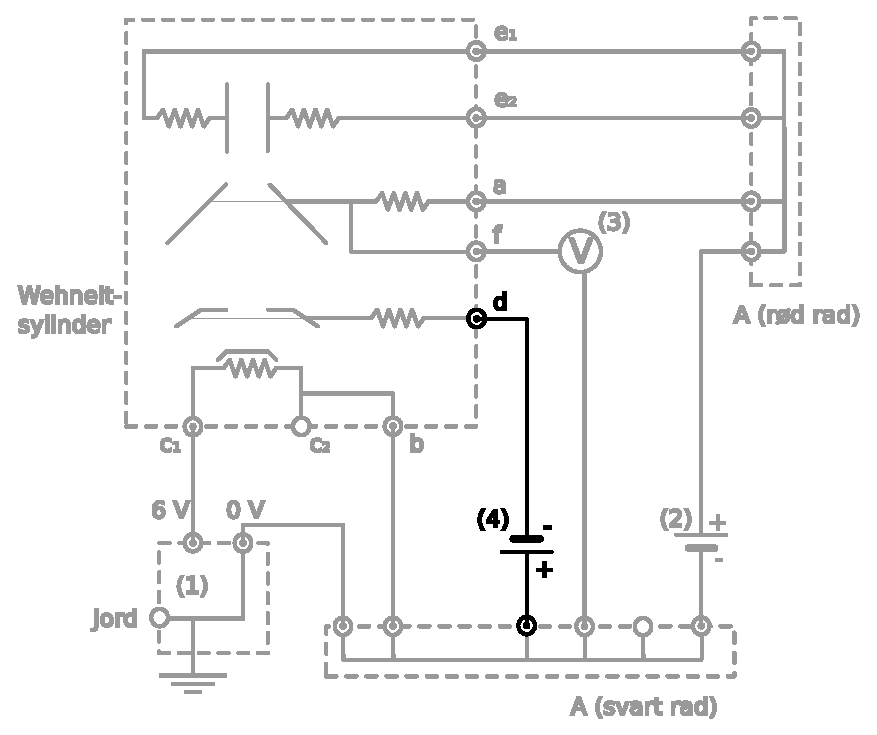
\includegraphics[width=0.6\textwidth]{fig/wehnelt.eps}
%\caption{\small\sf Kretsdiagram for elektronkanonen, steg 3: tilkopling av Wehneltsylinderen. De delene av diagrammet som har lysere farge er allerede oppkoplet i de foregående figurene; se forøvrig figur \ref{fig:glodekrets} og \ref{fig:anodespenning} for forklaring. (4) representerer en Mascot 719 kraftforsyning.}
%\label{fig:wehnelt}
%\end{center}
%\end{figure}




{\itsf Nå er det klart til å skru på alle spenninger og se at elektronstrålen vises:}
\vspace{-4mm} 
\begin{itemize}
\item Be labveilederen om å godkjenne oppkoplingen.
\item Slå spenningen for glødingen på.
\item Sjekk at filamentet starter å gløde.
%\item Kraftforsyningen (2) for akselerasjonsspenningen skal også være spenningsstyrt: Sett METER til V, skru på og sett strømknappen 1/4 omdreining opp.
\item Øk akselerasjonsspenningen sakte inntil du (ved 20--30 V eller noe høyere hvis øynene ikke har vent seg til mørket) ser 
sporet etter elektronstrålen i hydrogengassen som en blåfiolett stripe ut av elektronkanonen.
\item Observer hvordan strålen forandrer seg når du forandrer akselerasjonsspenningen.
\item Hvorfor når ikke strålen glassveggen ved lav akselerasjon? Ved høyere spenninger vil, ganske brått, strålen møte veggen, senk da spenningen noe. Dette skjer ved ulike spenninger ved de ulike oppsett, følg godt med rundt 100 V, og evt. oppover til ca. 150 V.
\item MERK: Hvis anoden begynner å gløde må du slå apparaturen av og la den avkjøle seg. Bruk aldri høyere akselerasjonsspenning enn nødvendig for å unngå gløding. 
\end{itemize}

{\itsf Lag en skisse av strålegangen for forskjellige akselerasjonsspenninger.}
%


Prosedyre for å \textbf{slå av apparaturen}:
\vspace{-4mm} 
\begin{itemize}
\item Slå glødespenningen av.
\item Reduser akselerasjonsspenningen til null og slå kraftforsyningen av. 
%\item Reduser fokuseringsspenningen til null og slå kraftforsyningen av.
\end{itemize}
MERK: Det er ikke farlig å ha på akselerasjonsspenning og magnetfelt uten å ha på glødespenning, men det er ikke bra å ha på glødespenning uten akselerasjonsspenning. Slå derfor alltid av glødespenningen når du har korte og lengre pauser.

I en elektronstråle har alle partiklene samme fortegn på ladningen. Strålen vil derfor ha en tendens til å divergere pga. intern Coulombkraft. Hvis fokuseringsringen (Wehneltsylinderen) foran katoden legges svakt negativt, vil dette virke fokuserende på strålen. 

{\itsf Kople til Wehneltsylinderen i henhold til figur \ref{lorentz.fig7}.}
Utgång 1 till "W".
Merknader og tips:
\vspace{-4mm} 
\begin{itemize}
    \item Sjekk at kraftforsyningen er slått av og at justeringsknappene for strøm og spenning er skrudd helt ned før du kobler den til.
    \item Etter du har koblet til Wehneltsylinderen og slått på kraftforsyningen. Juster spenningen på fokuseringselektroden (Wehneltsylinderen) hvis du synes at strålen er dårlig fokusert. Bruk maksimalt \SI{10}{\volt}.
\end{itemize}
\newpage

\subsection{Avbøyning i \textsl{E}-felt}
%%%%%%%%%%%%%%%%%%%%%%%%%%%%%%%%%%%%%%%%%

Oppgave:\\
{\itsf Du skal studere avbøyningen av en elektronstråle i et elektrostatisk felt.}

I oppstillingen til nå har du lagt begge avbøyningsplatene på samme spenning, nemlig anodespenningen $U_\mathrm{a}$. For å få avbøyning legges den ene plata på noe lavere spenning. I praksis gjør vi dette ved å ta spenningsdeling fra anodespenningen. Prinsippet for spenningsdeling er vist i figur \ref{lorentz.fig3}. Her må du gjøre forandringer i oppkoplingen. Anodespenningen (3) skal nå kobles med koblingsboks enligt skjemaet i figur \ref{fig:spenningsdeler} viser forandringer du må gjøre fra oppkopling i figur \ref{lorentz.fig7} der avbøyningspotensialet var null. Koblingen mellan e$_1$ och e$_2$ tas bort. 


Spenningsdeleren består av et presisjonspotensiometer (Helipot) og er montert på koplingsboks B. Akselerasjonsspenningen $U_\mathrm{a}$ koples over potensiometeret. Fra midttappingen tar vi ut en spenning som varierer med stillingen til potensiometerknappen, som trenger 10 omdreininger for å skrus fra topp til bunn. Avbøyningsspenningen tas ut mellom topputtaket (som altså er på potensial $U_\mathrm{a}$ ) og midtuttaket på potensial $x  U_\mathrm{a}$, der $x$ kan variere fra 0 til \SI{100}{\percent}. Det betyr at den ene avbøyningsplata ligger på anodespenningen $U_\mathrm{a}$ og den andre på $x  U_\mathrm{a}$. Avbøyningsspenningen blir da 
\begin{equation}
    U_\mathrm{d} 
        = U_\mathrm{a} - x U_\mathrm{a} 
        = (1 - x) U_\mathrm{a}.
\end{equation}
Hvis du kopler feil og tar ut spenningsdeling til jordpotensialet vil elektronstrålen bremses kraftig og lett forsvinne. Hvilken plate som skal ha lavere potensial finner du ut ved å tenke, eller ved å prøve og feile.

{\itsf Kople til avbøyningspotensialet ifølge figur \ref{fig:spenningsdeler}.}
 
\begin{figure}[!ht]
    \begin{center}
    \includegraphics[width=0.6\textwidth]{fig/spenningsdeler-new.pdf}
    \caption{%
        Kretsdiagram for inkopling av spenningsdeler.
    }
    \label{fig:spenningsdeler}
    \end{center}
\end{figure}

Merknader og tips:
\vspace{-4mm} 
\begin{itemize}
    \item Innstill potensiometeret på \SI{100}{\percent} slik at midttappingen har samme potensial som anodespenningen.
    \item Slå på glødingen, fokuseringsspenning og akselerasjon som beskrevet tidligere.
    \item Varier avbøyningen ved å skru på potensiometerknappen.
\end{itemize}

{\itsf Forklar det du observerer ut i fra uttrykket for Lorentzkraften i likning \eqref{eq:lorentz.lorentz}. 

Skisser strålen for forskjellige avbøyningsspenninger, f.eks. $U_\mathrm{d}$ lik $\half  U_\mathrm{a}$ og $\frac{4}{5} U_\mathrm{a}$.
}

 
\subsection{Avbøyning i \textsl{B}-felt}
%%%%%%%%%%%%%%%%%%%%%%%%%%%%%%%%%%%%%%%%%

Oppgave:\\
{\itsf Du skal studere avbøyningen av en elektronstråle i et statisk magnetfelt.}


{\itsf Kople oppstillinga i henhold til figur \ref{lorentz.fig7}.  Merk at oppkoplingen av spenningsdeleren i forrige steg ikke er nødvendig for forsøkene som skal utføres her}

{\itsf Kople strømkretsen til magnetene med Mascot aggregatet i (g)
.}

%\begin{figure}[!ht]
%    \begin{center}
%    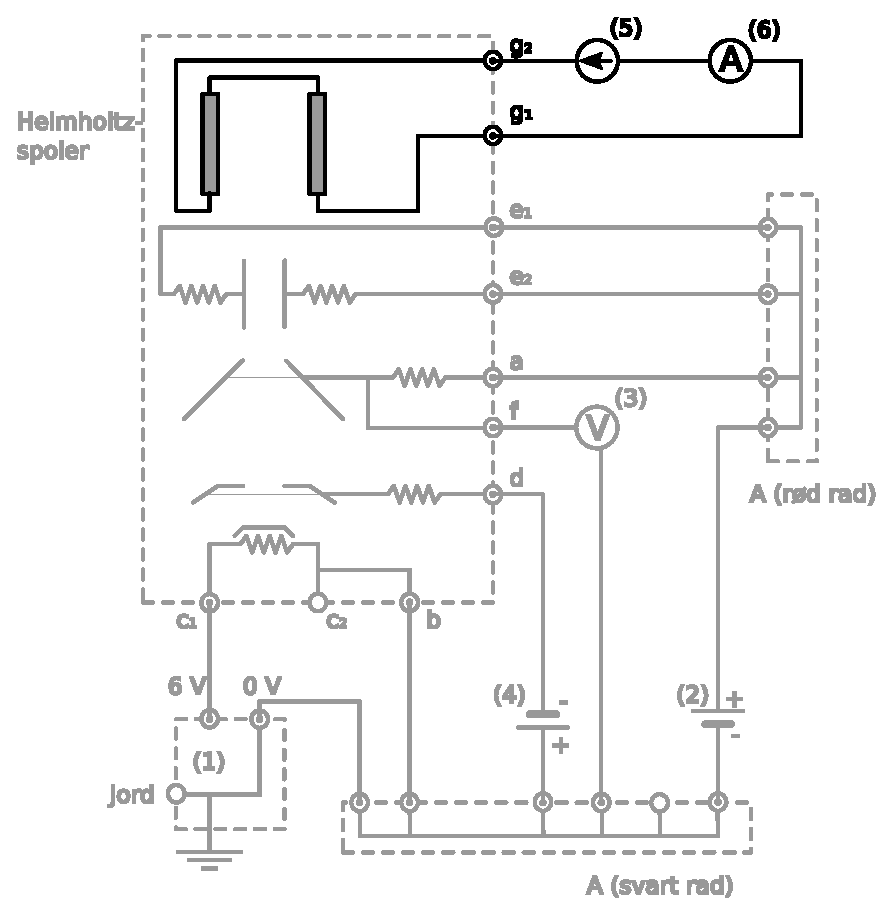
\includegraphics[width=0.6\textwidth]{fig/magnetfelt.eps}
%    \caption{%
%        Kretsdiagram for elektronkanonen, steg 5: tilkopling av Helmholtzspolene. De delene av diagrammet som har lysere farge er allerede oppkoplet i de foregående figurene; se forøvrig figur \ref{fig:glodekrets}, \ref{fig:anodespenning} og \ref{fig:wehnelt} for forklaring. 
%        (5) representerer en Mascot 719 kraftforsyning som strømkilde og 
%        (6) representerer et multimeter for måling av strømstyrken. Merk at oppkoplingen av spenningsdeleren i forrige steg (figur \ref{fig:spenningsdeler}) ikke er nødvendig for forsøkene som skal utføres her, og den er derfor ikke inkludert i dette diagrammet. Legg merke til at kretsen for Helmholtzspolene er uavhengig av resten av oppkoplingen.
%    }
%   \label{fig:magnetfelt}
%    \end{center}
%\end{figure}

Merknader og tips:
\vspace{-4mm} 
\begin{itemize}
    \item Sjekk at kraftforsyningen for Helmholtzspolene er avslått og at kontroll\-knappene for strøm og spenning er skrudd helt ned.
    \item Innstill kraftforsyningen til strømkilde (METER: A og reguleringsknappen for spenning opp 1/2 omdreining) og sett RANGE til \SI{15}{\volt}.
    \item Bruk multimeteret (6) for strømmåling
    \item Skru opp strømmen til ca. \SI{1}{\ampere}, og sjekk at strømkretsen virker. MERK: Spolene tåler maks. \SI{2}{\ampere}. Skru deretter strømmen ned igjen.
    \item Slå på elektronstrålen som beskrevet tidligere.
    \item Juster akselerasjonsspenningen til ca: \SI{100}{\volt} og magnetstrømmen til \SI{0,75}{\ampere}.
\end{itemize}

{\itsf Gi en forklaring på det som skjer forankret i uttrykket for Lorentzkraften. }

Be labveilederen om å hjelpe deg å vri elektronstrålerøret i opplagringen inntil strålen beskriver en heliksformet bane.

{\itsf Skisser strålen og forklar grunnen til den heliksformede banen.}

\subsection{Thomsoneksperimentet: måling av \textsl{e/m}}
%%%%%%%%%%%%%%%%%%%%%%%%%%%%%%%%%%%%%%%%%

Oppgave:\\
{\itsf Du skal bestemme forholdet $e/m$ mellom elektronets ladning og masse fra likning \eqref{eq:lorentz.7} ved å måle akselerasjonsspenningen $U_\mathrm{a}$, radien $r$ i elektronbanen og magnetfeltet $B$.}

Magnetfeltet er forhåndskalibrert mot strømmen i spolene. Resultatet er gitt i en kalibreringskurve vedlagt apparaturen og som et empirisk uttrykk for magnetfeltet som funksjon av målt spolestrøm funnet fra kalibreringskurven. Alternativt kan dette uttryck brukas:
\begin{equation}
    B=\mu_0 \cdot (\frac{4}{5})^{3/2}\cdot \frac{n}{R} \cdot I
\end{equation}
R: Spolenes radie, n: antal varv = 130 per spole.

Merknader og tips:
\vspace{-4mm} 
\begin{itemize}
    \item Rett opp røret slik at strålen blir en sirkel og ikke en heliks.
    \item Innstill multimeteret for spenningsmåling i området 0-\SI{1000}{\volt} likespenning.
    \item Be labveilederen om å vise deg hvordan du måler elektronbanens diameter ved hjelp parallakse-speilet bak elektronstrålerøret og en linjal.
    \item Det er mulig å fotografere elektronbanen og analysere i TRACKER for å få banens diameter. Observer at man må ha en skala (linjal) i bilden då.
\end{itemize}

\subsubsection{Analyse og diskusjon av Thomsoneksperimentet}
%%%%%%%%%%%%%%%%%%%%%%%%%%%%%%%%%%%%%%%%%

\vspace{-4mm} 
\begin{itemize}
    \item Bestem $e/m$ for elektronet ut i fra dine målinger av $U_\mathrm{a}$, $r$, $I$ og kalibreringskurven eller formeln for $B(I)$.
    \item Gjenta dersom du har tid bestemmelsen for et annet sett av verdier for $U_\mathrm{a}$ og $I$.
    \item Anslå feilene i de målte størrelser og finn målfeilen i $e/m$. 
    %\item 
    Hvilke feilkilder dominerer? 
    \item Sammenlign den målte verdi av $e/m$ med tabellverdi.
    \item Hvordan er overenstemmelsen mellom måleresultatene fra ulike verdier av $U_\mathrm{a}$ og $I$ og feilestimatet ditt?
    \item Diskuter mulige anvendelser av de fysiske effekter som er tatt opp til observasjon i eksperimentet.
\end{itemize}

%%%%%%%%%%%%%%%%%%%%%%%%%%%%%%%%%%%%%%%%%%%%%%%%%%
\subsection{Avslutning}
%%%%%%%%%%%%%%%%%%%%%%%%%%%%%%%%%%%%%%%%%%%%%%%%%%
Slå av alle apparater, trekk ut og rydd opp i alle ledninger. Forlat plassen i minst like god orden som du fant den.


\end{document}